\chapter{Diseño y arquitectura del sistema}
\label{capitulo3}
\lhead{Capítulo 3. \emph{Diseño del sistema}}

En este capitulo se explicará la arquitectura, el diseño y el modo en el que el IDS basado en SSM interactuara con Bro. Además, se detallaran las salidas y los datos de configuración que va a considerar el sistema para su correcto funcionamiento vas a considerar. Este capitulo tiene la intención de mostrar la visión general del modelado del sistema que se realizo a partir de las bases teóricas.

\section{Arquitectura del sistema}

La arquitectura del detector de intrusiones que se muestra en el presente trabajo se basa en una arquitectura modular la cual está conformada por tres modulo. Un modulo para realizar la segmentación de los URIs, otro  para realizar la evaluación y un tercero para realizar el entrenamiento y de esta forma crear un modelo de normalidad.

A grandes rasgos, el modulo de segmentación se encargará de tomar el URI que proviene de la solicitud de tipo GET o HEAD que se le hace al servidor HTTP, normalizarlo y segmentarlo siguiendo las especificaciones del RFC (insertar nombre del RFC) .

Por otra parte, el modulo de evaluación se encargará de evaluar la probabilidad de generación de cada uno de los segmentos del URI generados por el modulo de segmentación para al final decidir si el URI de la solicitud enviada al servidor de tipo HTTP es anómalo o no.

Por último, el modulo de entrenamiento será el encargado de crear el modelo de normalidad del sistema. Para esto, el sistema recibirá solicitudes libres de ataques e irá calculando la probabilidad de aparición de cada una de las palabras que aparecen en las mismas.

Tanto el modulo de evaluación, como el modulo de entrenamiento son dependientes del modulo de segmentación ya que requieren de los segmentos de URI generados por eso para realizar su trabajo. 

La arquitectura del sistema queda detallada en la figura \ref{fig:arquitectura}.

\begin{figure}[tb]
\begin{center}
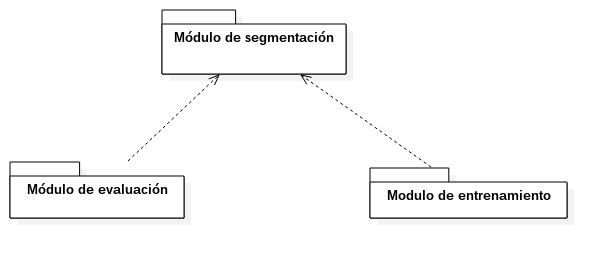
\includegraphics[width=3in]{arquitectura.png}
\caption{Arquitectura del sistema.}
\label{fig:arquitectura}
\end{center}
\end{figure}

\begin{itemize}
\item Modo evaluación: En este modo de operación solo se activaran los módulos de segmentación y evaluación del sistema. A manera general, esta modalidad, se encargará de recibir peticiones de tipo HTTP/GET, extraer su URI y segmentarlos a tráves del modulo de segmentación para luego evaluar si  el mismo es anómalo o no, haciendo uso del modulo de evaluación. El funcionamiento de esta modalidad queda detallado en la figura \ref{fig:modoSistema}.
\item Modo entrenamiento ``Online'': En este modo de operación solo trabajaran los módulos de segmentación y entrenamiento. Esta modalidad es un tipo de entrenamiento en donde se toman peticiones de tipo HTTP/GET y se segmenta el URI que se encuentran en las mismas haciendo uso del modulo de segmentación. Una vez realizado esto, el modulo de entrenamiento tomara los segmentos arrojados por el modulo de segmentación, calculara la probabilidad de aparición de los mismos para de esta manera ir modificando un modelo de normalidad previamente establecido, es decir, la salida de este modo de entrenamiento sera la de el modelo previamente establecido con ciertas modificaciones realizadas a partir de las observaciones hechas. El funcionamiento de esta modalidad queda detallado en la figura \ref{fig:modoSistema}..
\item Modo entrenamiento ``Offline'': Esta modalidad del sistema en análoga al modo de entrenamiento ``Online''. El único aspecto que diferencia a ambas modalidades es que cuando el sistema funciona en modo ``Offline'' no se toma en cuenta, ni se modifica un modelo de normalidad previamente construido. La salida de este modo de entrenamiento sera un modelo de normalidad construido desde cero.El funcionamiento de esta modalidad queda detallado en la figura \ref{fig:modoSistema}.
\end{itemize}

\begin{figure}[tb]
\begin{center}
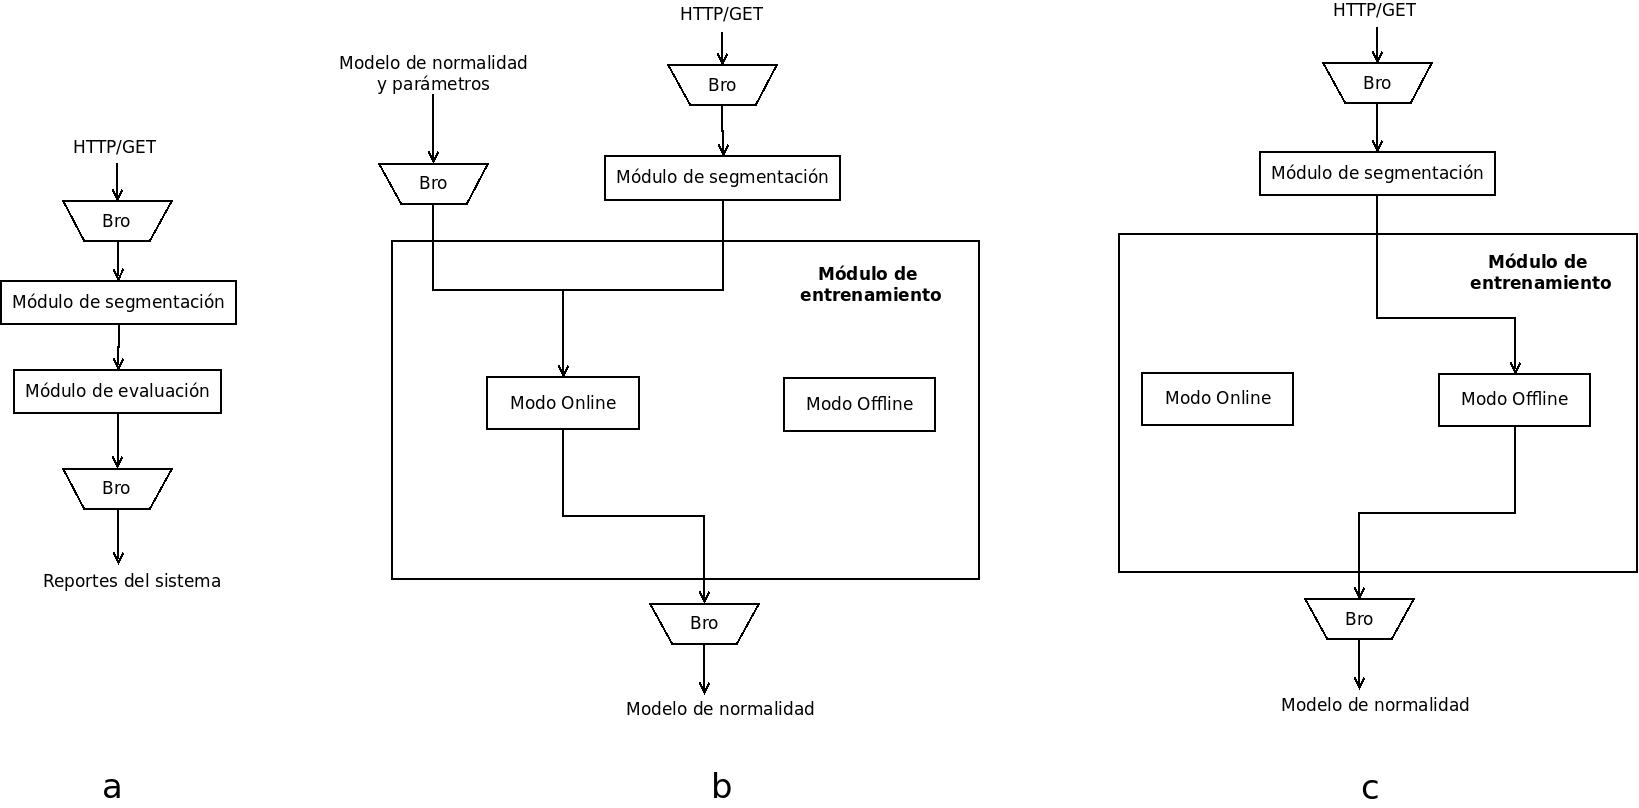
\includegraphics[width=\linewidth]{modoOperacion.jpeg}
\caption{Modo evaluación (a), modo entrenamiento ``Online'' (b), modo entrenamiento ``Offline'' (c).}
\label{fig:modoSistema}
\end{center}
\end{figure}

\section{Módulos}

En esta sección se describirán las tareas de cada uno de los módulos que conformar la arquitectura detallada en la figura \ref{fig:arquitectura}, el modo en el que se subdividieron dichas tareas, los datos de entrada y salida, y la interacción que existe entre los mismos.

\subsection{Modulo de segmentación}

El modulo de segmentación es un elemento clave dentro de la construcción del IDS basado en SSM, es por eso que su buen diseño e implementación es importante para el buen funcionamiento del sistema. Este se encarga, como se menciono anteriormente,de tomar el URI que proviene de la solicitud de tipo GET o HEAD que se le hace al servidor HTTP capturado por Bro, normalizarlo y segmentarlo siguiendo las especificaciones del RFC (insertar nombre del RFC) 

Es evidente entonces, que este modulo consta de dos funcionalidades fundamentales: la normalización de los URIs y la segmentación.  La normalización se encargará de tomar el URI de las peticiones HTTP entrantes y codificarlo a formato UTF-8. Normalizar es un paso importante dentro del sistema  ya que se estandarizar la forma en las que están escritos los URIs facilita tanto la evaluación como el entrenamiento en el sistema. Por otra parte, el output arrojado por esta función de normalización será tomado por la de segmentación, quien a su vez se encargará de segmentar el URI de la forma en la que se explica en la sección \ref{sec:delimitadores}, es decir, el URI se dividirá en las diferentes partes estipuladas en el RFC 3986: el ``host'', la ruta, los argumentos, los valores y el ``fragment''.

 En las base teórica, la segmentación de los URIs se realiza mediante un autómata que se encarga de reconocer (realizar un análisis sintáctico) y evaluar en cada uno de sus estados la probabilidad de generación de cada uno de los segmentos.  No obstante, en la función de segmentación del sistema implementado, esta tarea se modeló mediante un analizador sintáctico que hace uso de una gramática (libre de contexto) de atributos que genera el mismo lenguaje que reconoce el autómata presentado en la figura ~\ref{fig:automata}, es decir, el lenguaje de los URI.

En la figura \ref{fig:arquiSegmentacion} se puede apreciar el diagrama de bloques que refleja el funcionamiento del módulo de segmentación.

\begin{figure}[tb]
\begin{center}
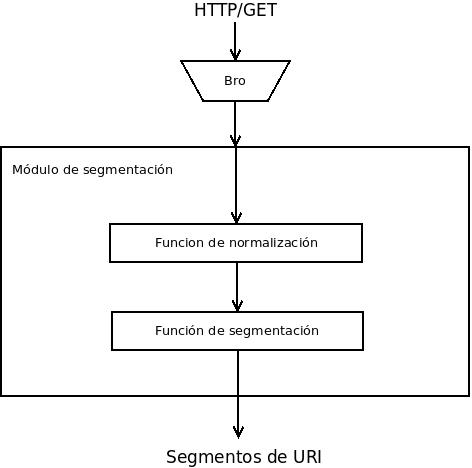
\includegraphics[width=3in]{segArquiCompleta.jpeg}
\caption{Diagrama de bloques del módulo de segmentación.}
\label{fig:arquiSegmentacion}
\end{center}
\end{figure}

\subsection{Modulo de evaluación}
\label{sec:evaluacion}

El módulo de evaluación, es el encargado de evaluar la probabilidad de generación de cada uno de los segmentos del URI otorgados por el modulo de segmentación, dado un modelo de normalidad. Una vez calculadas estas probabilidades, el modulo se encargará de calcular un índice de anormalidad del URI mediante el uso de las formulas descritas en la sección ~\ref{subsec:exprIndice} para luego compararlo con un parámetro $\theta$ (\ref{eq:ClaseU}) y de este modo saber si los segmentos de URI que ingresaron como entrada posee alguna anormalidad o no. Luego de realizar esta evaluación, el modulo se encargara de escribir los reportes del sistema en un ``log''.

El módulo de evaluación, está conformado por dos grandes funcionalidades: una que se encargará de leer el modelo de normalidad y  otra que calculará el índice de anormalidad y evaluará si el mismo es anómalo o no. 

**Función de lectura de datos:
El modelo teórico que fue explicado en la sección ~\ref{sec:modeloSSM} posee elementos como: un conjunto “S” de estados, un conjunto “O” de símbolos observables que se encuentran en cada estado, una matriz “A” que contiene la probabilidad de transición entre estados, un conjunto “B” de vectores que contiene la probabilidad de las palabras observadas en cada estado y un vector de probabilidades iniciales. No obstante, los únicos elementos del modelo que se necesitan ingresar en el sistema para que este funcione y realice las tareas de evaluación son: el conjunto “O” de símbolos observables que se encuentra en cada estado y el conjunto de vectores “B”. El conjunto “B” es necesario para resolver la expresión \ref{eq:sumB}. Por otra parte, es necesario hacer uso tanto de “B” como “O” para obtener el valor de $b_{qtot}$ presentado en la ecuación \ref{eq:Pqtot}. Este elemento es sumamente importante para calcular el índice de anormalidad. Por otra parte, será necesario introducir al sistema los valores de probabilidad de fuera de vocabulario (Poov), ya que son necesarios para obtener el valor de $p_{qtot}$, presente en la ecuación \ref{eq:Pqtot}, en caso que una cadena de caracteres del URI que se esté analizando no se encuentre en el conjunto de observaciones “O”. Además, se requiere el valor del parámetro $\theta$ para evaluar el índice de anormalidad según lo estipulado en la ecuación \ref{eq:ClaseU} .

    Entonces, en conclusión, los parámetros que requieren ser introducidos al sistema de detección de intrusiones para que este funcione de manera correcta son: el conjunto de observaciones de cada estado (O), el conjunto de vectores de probabilidad de las palabras observadas en cada estado ( $B_{S}, B_{P}, B_{A}, B_{V}$ ), los valores de probabilidad de fuera de vocabulario, es decir $P_{oovS}, P_{oovP}, P_{oovA}, P_{oovV}$ y el valor del parámetro $\theta$. Todos estos parámetros serán leídos por la función de lectura del modulo de evaluación.
    
Una vez leídos los parámetros necesarios para que el sistema funcione, estos serán enviados a la función de evaluación junto a los segmentos de URI dados por el módulo de segmentación. Una vez recibidos los datos de entrada, esta función se encargará de hallar el índice de anormalidad ($N_{s}$) mediante la expresión \ref{eq:Ns} para, de este modo compararlo con el parámetro $\theta$ como se indica en \ref{eq:ClaseU}.No obstante, las tareas de calculo y evaluación del índice de anormalidad, fueron subdivididas a su vez, en cuatro funciones. La primera de las funciones será la encargada de calcular tanto el $\varepsilon_{0}$ que aparece en la expresión \ref{eq:sumB} como la sumatoria de los logaritmos de los $p_{qtot}$ que se encuentra en \ref{eq:Ns}; la segunda función tomará el valor de $\varepsilon_{0}$ y la sumatoria de los logaritmos de los $p_{qtot}$ que calculó la primera función y procederá a efectuar todas las operaciones que hay en la expresión \ref{eq:Ns} para de este modo obtener el índice de anormalidad, $N_{s}$; por otra parte, la tercera función tendrá como tarea comparar el índice de anormalidad $N_{s}$ calculado por la tercera función, con el parámetro $\theta$ como se indica en \ref{eq:ClaseU}; la cuarta será la encargada de escribir en un archivo de texto aquellos URIs anómalos.

El diagrama de bloques presente en la figura \ref{fig:arquiEvaluacion} representa el funcionamiento del módulo de evaluación.

\begin{figure}[tb]
\begin{center}
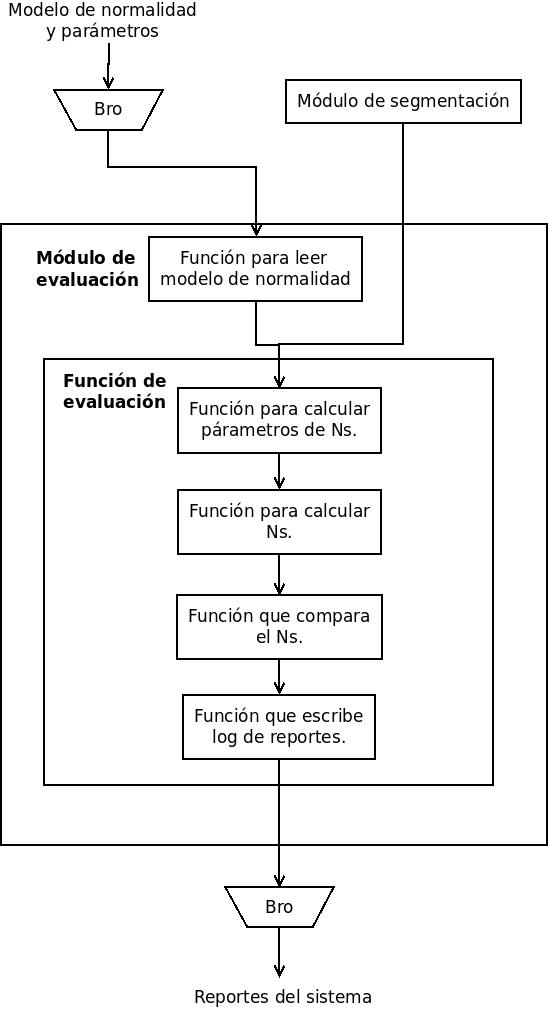
\includegraphics[width=3in]{evalArqui.jpeg}
\caption{Diagrama de bloques del módulo de evaluación.}
\label{fig:arquiEvaluacion}
\end{center}
\end{figure}

\subsection{Modulo de entrenamiento}\label{sec:entrenamiento}

El modelo de normalidad es uno de los aspecto importantes dentro del IDS basado en SSM ya que a partir de la información que este almacena se podrá decidir si un URI es anómalo o no dependiendo de la similitud que posea este con los datos que almacena el modelo. Por esta razón, realizar un modelo de normalidad apropiado es un aspecto  importante para que el módulo de evaluación haga detecciones de intrusiones más certeras.

El módulo encargado de elaborar los modelos de normalidad será el módulo de entrenamiento. A grandes rasgos, este se encargará de recibir un conjunto de segmentos libres de ataques proporcionados por el módulo de segmentación para ir calculando la probabilidad de aparición de cada una de las palabras que aparecen en los mismos, para finalmente, escribir en un archivo toda la información recolectada, es decir, el conjunto de palabras observadas mientras se hacía el entrenamiento, sus probabilidades de aparición y el estado del autómata en el que se observaron las mismas.

Este módulo consta de dos modos: el modo ``Offline'' y el modo ``Online''. La  diferencia fundamental entre el modo ``Online'' y el ``Offline'' es que en el primero necesita como entrada un modelo de normalidad ya construido y los segmentos de URI proporcionados por el módulo de segmentación. Una vez realizado el entrenamiento, esta modalidad se encargará de actualizar el modelo que se leyó al inicio. Por otra parte, el modo ``Online'' solo requiere como entrada los segmentos de URI y como salida proporcionará un  modelo de normalidad construido desde cero.

El modo de entrenamiento ``Online'' fue dividido en tres funciones. La primera función irá observando los segmentos de los URIs de las peticiones que van llegando y contará el numero de veces que cada segmento fue observado durante el entrenamiento. La segunda función, toma el resultado de las observaciones realizadas por la primera función y calculará la probabilidad de aparición de cada uno de los segmentos haciendo uso de la formula \ref{eq:entrenamiento}. La tercera función tomara los resultados otorgados por la segunda función y los escribirá en un archivo de texto. Este archivo representara el modelo de normalidad construido.

Por otra parte, las tareas a realizar por el modo de entrenamiento ``Offline'' fueron divididas de igual modo en tres funciones: La primera función se encargara de leer el modelo de normalidad; la segunda se encargará de tomar el modelo de normalidad leído por la primera función y el conjunto de segmentos de URI del módulo de segmentación. Esta información sera utilizada por la misma para ir calculando la probabilidad de aparición de los segmentos observados. La tercera función se encargara de recibir los resultados obtenidos por la segunda función y actualizara el modelo de normalidad previamente existente.

En la figura {fig:arquiEntrenamiento} se puede apreciar el diagrama de bloques que describe el funcionamiento del módulo de entrenamiento.

\begin{figure}[tb]
\begin{center}
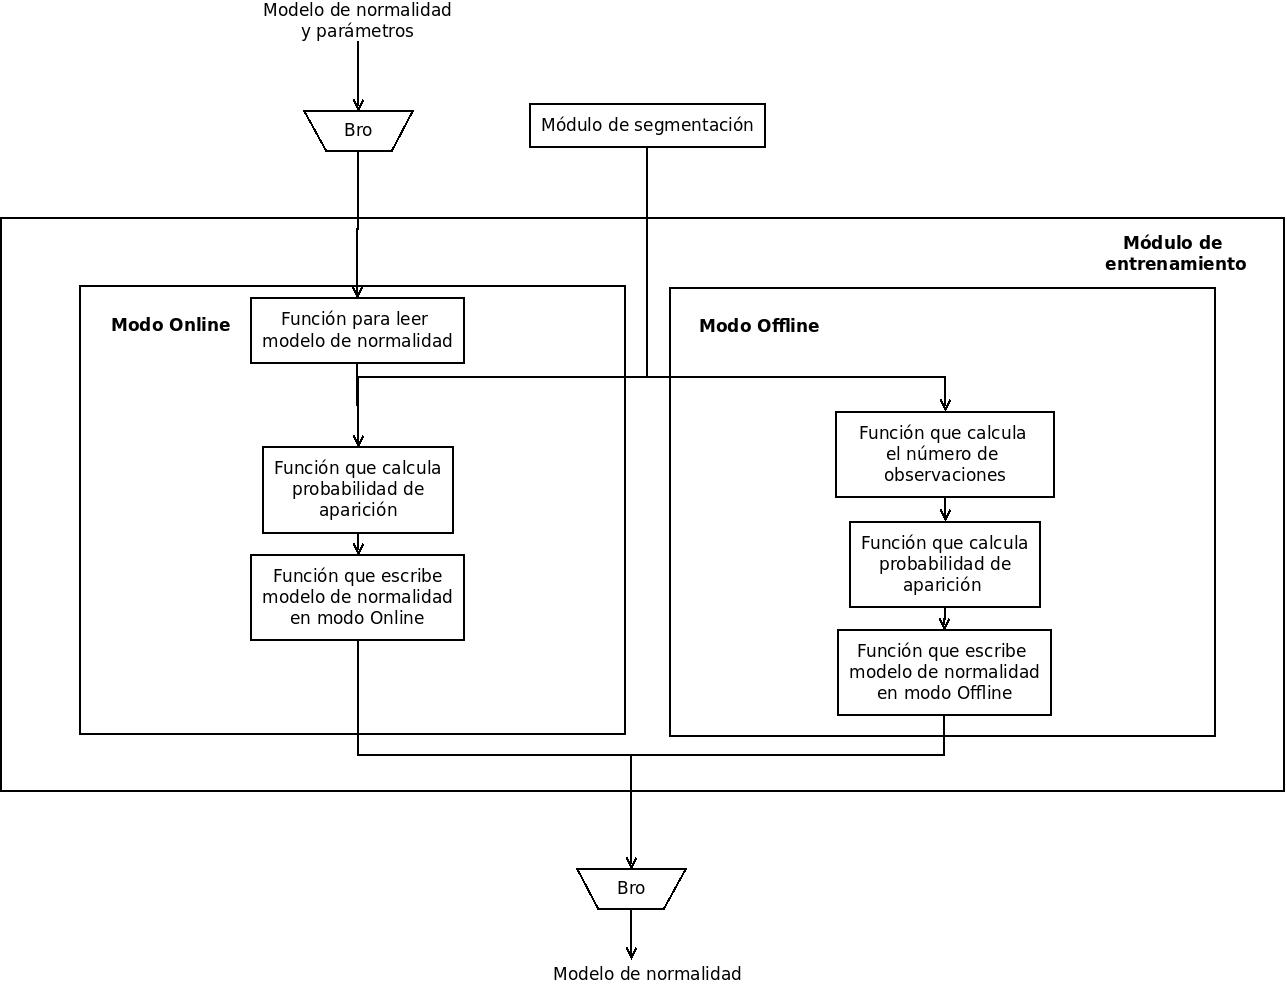
\includegraphics[width=4in]{entrenamArqui.jpeg}
\caption{Diagrama de bloques del módulo de entrenamiento.}
\label{fig:arquiEntrenamiento}
\end{center}
\end{figure}

*********************************************************************

El entrenamiento en modo “Offline” se encargará de tomar los segmentos de un flujo de URIs sin anomalías, contar el número de aparición de cada uno de los segmentos de los URIs, para luego calcular la probabilidad de aparición de cada uno de ellos. Una vez culminadas estas tareas se procederá a escribir en un archivo toda la información recolectada, es decir, el conjunto de palabras observadas mientras se hacía el entrenamiento, sus probabilidades de aparición y el estado del autómata en el que se observaron las mismas.

Por otra parte, el modo de entrenamiento en modo “Online” a diferencia del entrenamiento en modo “Offline” necesita como entrada: un flujo de segmentos de URIs proporcionados por el modulo de segmentación y un archivo con un modelo de normalidad ya construido. Esta función, se encargará de ir modificando el modelo de normalidad ingresado a medida que se vayan recibiendo nuevos segmentos de URI para de esta manera construir el nuevo modelo.










finalmente el conjunto de palabras observadas mientras se hacía el entrenamiento, sus probabilidades de aparición y el estado del autómata en el que se observaron las mismas

dar al sistema una lista de palabras observadas junto con su probabilidad de aparición.

``Este módulo de entrenamiento será el encargado de armar el vocabulario del módulo de normalidad del sistema. Como se mencionó con anterioridad, este módulo tomará un conjunto de solicitudes libres de ataques, para luego calcular la probabilidad de aparición de las palabras en el conjunto de observaciones totales de cada uno de los estados. En términos más formales, la  tarea que realiza este módulo se puede modelar de la siguiente forma:''

``La implementación del módulo de entrenamiento consta de dos modos, el modo “Offline” y el modo “Online”. El entrenamiento en modo “Offline” se encargará de tomar los segmentos de un flujo de URIs sin anomalías, contar el número de aparición de cada uno de los segmentos de los URIs, para luego calcular la probabilidad de aparición de cada uno de ellos. Una vez culminadas estas tareas se procederá a escribir en un archivo toda la información recolectada, es decir, el conjunto de palabras observadas mientras se hacía el entrenamiento, sus probabilidades de aparición y el estado del autómata en el que se observaron las mismas.

Por otra parte, el modo de entrenamiento en modo “Online” a diferencia del entrenamiento en modo “Offline” necesita como entrada: un flujo de segmentos de URIs y un archivo con un modelo de normalidad ya construido. Esta función, se encargará de ir modificando el modelo de normalidad ingresado a medida que se vayan recibiendo nuevos segmentos de URI para de esta manera construir el nuevo modelo.''